\begin{figure*}[!htb]
    \centering
    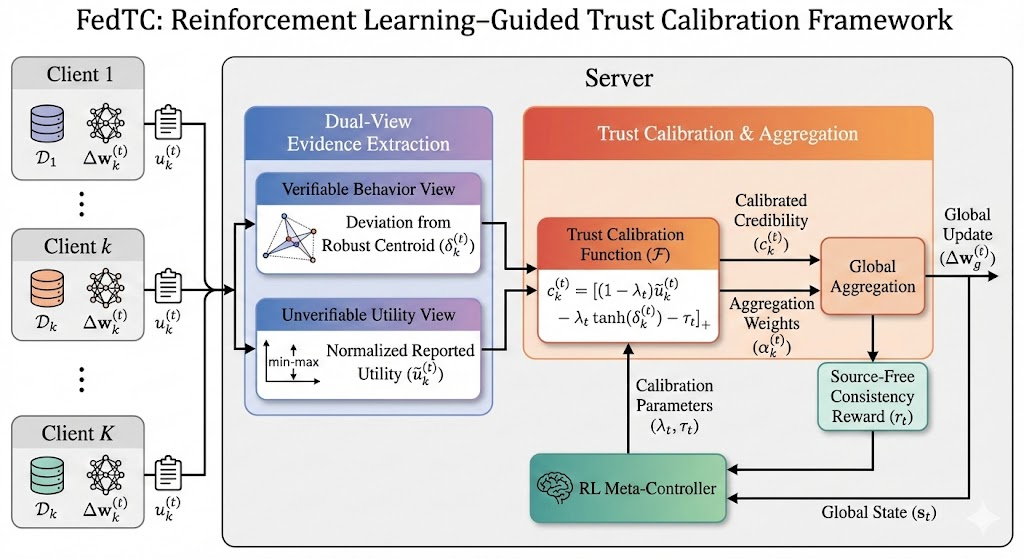
\includegraphics[width=0.8\linewidth]{content/figs/FedTC_framework.jpg}
    \caption{\textbf{Historical FedTC framework illustration (pending update).} The forward--backward organization motivates the current method, but the image retains earlier utility-normalization, calibration-function, and reward labels. The current rank normalization, calibration equation, interval feedback, and fallback gate are defined in Section~\ref{sec:method}; the image is not an exact specification of the released implementation or evidence of experimental performance.}
    \label{fig:framework}
\end{figure*}

\section{Method}
\label{sec:method}

We now present \textbf{FedTC} (Federated Trust Calibration), a server-data-free closed-loop framework for robust federated aggregation. At a high level, FedTC separates \emph{how updates are weighted in a single round} from \emph{how strict the filter should be over time}. We group the $T$ communication rounds into $N = T / H$ \emph{control macro-steps} $n \in \{0, \dots, N-1\}$, each spanning $H \ge 1$ consecutive rounds $\mathcal{T}_n = \{nH, \dots, (n+1)H - 1\}$. Within macro-step $n$, the server holds two interpretable calibration parameters $\mathbf{a}_n = (\lambda_n, \tau_n)$ fixed and runs the \emph{Forward Calibration Layer} every round; at the end of the macro-step, the \emph{Backward Confidence-Interval Controller} measures how the $H$-round model update affected honest clients---including rare minorities---and adjusts $\mathbf{a}_{n+1}$ accordingly.

\subsection{Aggregation as Trust Calibration}
\label{sec:agg_as_trust}

At round $t \in \mathcal{T}_n$, the server receives model deltas $\{\Delta\mathbf{w}_k^{(t)}\}_{k\in\mathcal{S}_t}$ and self-reported utilities $\{u_k^{(t)}\}_{k\in\mathcal{S}_t}$ from the sampled training cohort $\mathcal{S}_t$ ($|\mathcal{S}_t| = K_{\mathrm{train}}$). Instead of making a brittle keep-or-drop decision, FedTC assigns each client a continuous credibility score $c_k^{(t)} \ge 0$ and aggregates via normalized weights:
\begin{equation}
    \alpha_k^{(t)} = \frac{c_k^{(t)}}{\sum_{j\in\mathcal{S}_t} c_j^{(t)}},
    \qquad
    \Delta\mathbf{w}_g^{(t)} = \sum_{k\in\mathcal{S}_t} \alpha_k^{(t)} \Delta\mathbf{w}_k^{(t)},
    \label{eq:cred_based_agg}
\end{equation}
with $\mathbf{w}_{t+1} = \mathbf{w}_t + \Delta\mathbf{w}_g^{(t)}$ (and fallback $\Delta\mathbf{w}_g^{(t)} = \boldsymbol{\mu}_{\mathrm{rob}}^{(t)}$ if the denominator were ever zero, which Proposition~\ref{prop:non_collapse} rules out).

\subsection{Dual-View Dimensionless Evidence Extraction}
\label{sec:dual_view}

Raw gradient norms shrink naturally as training converges and vary widely across architectures. To make a single calibration rule work across all phases of training, FedTC converts both behavioral updates and client claims into dimensionless cohort-relative quantities.

\paragraph{Verifiable dimensionless deviation.}
The server first computes the geometric median via Weiszfeld's algorithm as a robust consensus anchor:
\begin{equation}
    \boldsymbol{\mu}_{\mathrm{rob}}^{(t)} = \operatorname*{arg\,min}_{\boldsymbol{\mu}\in\mathbb{R}^d} \sum_{k\in\mathcal{S}_t} \big\|\Delta\mathbf{w}_k^{(t)} - \boldsymbol{\mu}\big\|_2.
    \label{eq:geom_median}
\end{equation}
Unlike the arithmetic mean, the geometric median resists up to nearly half of the cohort being arbitrary outliers. Let $\delta_k^{(t)} = \|\Delta\mathbf{w}_k^{(t)} - \boldsymbol{\mu}_{\mathrm{rob}}^{(t)}\|_2$ be client $k$'s Euclidean distance from this anchor, and let $s_t = \operatorname{median}_{j\in\mathcal{S}_t} \delta_j^{(t)}$ be the typical spread of the round. Dividing by $s_t$ yields the \emph{dimensionless deviation}:
\begin{equation}
    \tilde{\delta}_k^{(t)} = \frac{\delta_k^{(t)}}{s_t + \varepsilon_s} \ge 0,
    \label{eq:delta_tilde}
\end{equation}
where $\varepsilon_s = 10^{-8}$ prevents division by zero. Intuitively, $\tilde{\delta}_k^{(t)} = 1$ means client $k$ sits at the median radius of the cohort, regardless of learning rate or training epoch.

\paragraph{Cohort-wise rank-normalized utility.}
Raw client utility claims $u_k^{(t)}$ cannot be compared directly across clients or trusted against extreme outliers (e.g., an adversary reporting $10^6$ would crush honest clients under min--max scaling). We therefore map $\{u_k^{(t)}\}_{k\in\mathcal{S}_t}$ to their intra-cohort ranks:
\begin{equation}
    \tilde{u}_k^{(t)} = \frac{\operatorname{rank}\!\big(u_k^{(t)} \text{ in } \mathcal{S}_t\big) - 1}{\max(K_{\mathrm{train}} - 1,\, 1)} \in [0, 1].
    \label{eq:u_norm}
\end{equation}
Together, $\mathbf{x}_k^{(t)} = (\tilde{u}_k^{(t)}, \tilde{\delta}_k^{(t)})$ pairs what client $k$ \emph{claims} with how far it \emph{strays} from the consensus.

\subsection{Forward Analytical Calibration Layer}
\label{sec:trust_calibration}

Given the macro-step action $(\lambda_t, \tau_t) = (\lambda_n, \tau_n)$ constrained to the explicit domain
\begin{equation}
\begin{aligned}
    \lambda_t &\in [0,\, \lambda_{\max}] \quad (\lambda_{\max} = 0.5), \\
    \tau_t &\in [\tau_{\min},\, \tau_{\max}] \quad (\tau_{\min} = 1.05,\; \tau_{\max} = 1.80),
\end{aligned}
    \label{eq:action_domain}
\end{equation}
and fixed temperature $\sigma_0 = 4.0$, FedTC computes the calibrated credibility score:
\begin{equation}
\begin{aligned}
    c_k^{(t)} &= \mathcal{F}\big(\mathbf{x}_k^{(t)}; \lambda_t, \tau_t\big) \\
    &= \Big[(1 - \lambda_t) + \lambda_t \tilde{u}_k^{(t)} - \tau_t \tanh\!\Big(\frac{\tilde{\delta}_k^{(t)}}{\sigma_0}\Big)\Big]_+,
\end{aligned}
    \label{eq:calibration}
\end{equation}
where $[x]_+ = \max(0, x)$. The two control knobs have clear physical roles: $\lambda_t$ governs how much weight the server places on client-reported utility (capped at $0.5$ so claims never dominate), while $\tau_t$ sets the geometric strictness---applying a smooth $\tanh$ penalty near the center and hard-truncating to zero beyond a finite radius.

Under~\eqref{eq:action_domain} and $\sigma_0 = 4.0$, the forward layer enjoys four exact analytical guarantees (proved in Appendix~\ref{app:proofs}):

\begin{proposition}[Non-Collapse of Central Clients]
\label{prop:non_collapse}
For any $(\lambda_t, \tau_t)$ satisfying~\eqref{eq:action_domain} and $\sigma_0 = 4.0$, at least $\lceil K_{\mathrm{train}} / 2 \rceil$ clients satisfy $\tilde{\delta}_k^{(t)} \le 1$, and each such central client attains
\begin{equation}
\begin{aligned}
    c_k^{(t)} &\ge (1 - \lambda_{\max}) - \tau_{\max} \tanh(1 / \sigma_0) \\
    &= 0.5 - 1.8\tanh(0.25) > 0.059.
\end{aligned}
    \label{eq:non_collapse}
\end{equation}
Consequently, $\sum_{j\in\mathcal{S}_t} c_j^{(t)} > 0.059 \lceil K_{\mathrm{train}} / 2 \rceil > 0$ holds unconditionally, guaranteeing exact convex combination weights $\sum_{k\in\mathcal{S}_t} \alpha_k^{(t)} = 1$.
\end{proposition}

\begin{lemma}[Monotonicity and Lipschitz Stability]
\label{lem:mono_lip}
For any fixed $(\lambda_t, \tau_t)$ in~\eqref{eq:action_domain}, $c_k^{(t)}$ is non-decreasing in $\tilde{u}_k^{(t)}$ and non-increasing in $\delta_k^{(t)}$, and satisfies the global Lipschitz bound
\begin{equation}
    \big|c(\tilde{u}_1, \tilde{\delta}_1) - c(\tilde{u}_2, \tilde{\delta}_2)\big|
    \le \lambda_t |\tilde{u}_1 - \tilde{u}_2| + \frac{\tau_t}{\sigma_0 (s_t + \varepsilon_s)} |\delta_1 - \delta_2|.
    \label{eq:lip_bound}
\end{equation}
\end{lemma}

\begin{proposition}[Exact Analytical Cutoff Radius and Bounded Aggregation Bias]
\label{prop:cutoff}
For any $\tau_t \in [\tau_{\min}, \tau_{\max}]$ (so $\tau_t > 1$) and any worst-case Fake Utility claim $\tilde{u}_k^{(t)} \in [0, 1]$, define the cutoff radius
\begin{equation}
    R_t(\tau_t) \triangleq \sigma_0 (s_t + \varepsilon_s) \operatorname{arctanh}\!\left(\frac{1}{\tau_t}\right).
    \label{eq:cutoff_radius}
\end{equation}
Whenever $\delta_k^{(t)} \ge R_t(\tau_t)$, we have $c_k^{(t)} = 0$ identically. Furthermore, the single-step deviation from the geometric median is strictly bounded:
\begin{equation}
    \big\|\Delta\mathbf{w}_g^{(t)} - \boldsymbol{\mu}_{\mathrm{rob}}^{(t)}\big\|_2 < R_t(\tau_t).
    \label{eq:agg_bias_bound}
\end{equation}
\end{proposition}

\begin{proposition}[Benign--Malicious Separation Condition]
\label{prop:separation}
Suppose in round $t$, honest clients satisfy $\tilde{\delta}_h^{(t)} \le \tilde{\delta}_{\max}^{\mathcal{H}}$ and malicious clients satisfy $\tilde{\delta}_b^{(t)} \ge \tilde{\delta}_{\min}^{\mathcal{B}} > \tilde{\delta}_{\max}^{\mathcal{H}}$. Whenever
\begin{equation}
    \frac{1}{\tanh(\tilde{\delta}_{\min}^{\mathcal{B}} / \sigma_0)} < \frac{1 - \lambda_t}{\tanh(\tilde{\delta}_{\max}^{\mathcal{H}} / \sigma_0)},
    \label{eq:sep_margin}
\end{equation}
any threshold $\tau_t$ in the non-empty interval $\big(\tanh^{-1}(\tilde{\delta}_{\min}^{\mathcal{B}}/\sigma_0),\, (1-\lambda_t)\tanh^{-1}(\tilde{\delta}_{\max}^{\mathcal{H}}/\sigma_0)\big) \cap [\tau_{\min}, \tau_{\max}]$ yields $c_h^{(t)} > 0$ for all $h \in \mathcal{H}\cap\mathcal{S}_t$ and $c_b^{(t)} = 0$ for all $b \in \mathcal{B}\cap\mathcal{S}_t$.
\end{proposition}

In plain terms, Proposition~\ref{prop:non_collapse} prevents total weight collapse, Proposition~\ref{prop:cutoff} ensures no adversary can buy influence outside $R_t(\tau_t)$ with fake utility claims, and Proposition~\ref{prop:separation} shows that a clean separating choice of $(\lambda_t, \tau_t)$ exists whenever honest and malicious updates are separated. The remaining question is: \emph{how should the server find and update $(\lambda_t, \tau_t)$ online without a clean validation set?}

\subsection{Backward Confidence-Interval RL Controller}
\label{sec:rl_meta}

To adapt $(\lambda_n, \tau_n)$ across changing non-IID cohorts and non-stationary attacks, FedTC closes the loop once every $H$ rounds. Grouping $H$ rounds into a macro-step serves two purposes: it lets meaningful loss changes accumulate above single-round stochastic noise, and it amortizes evaluation overhead by a factor of $H$.

\paragraph{True macro-step objective with bounded evaluation loss.}
A single corrupted batch or diverged local head can cause standard cross-entropy loss to explode, skewing any average. We therefore cap the per-sample evaluation loss at $M_{\mathrm{loss}} \ge \ln C_{\mathrm{cls}}$ via $\ell_{\mathrm{eval}}(\mathbf{w}; x, y) = \min(\ell_{\mathrm{CE}}(\mathbf{w}; x, y), M_{\mathrm{loss}})$. Over macro-step $n$ (moving from $\mathbf{w}_{nH}$ to $\mathbf{w}_{(n+1)H}$), client $i$'s true validation improvement on its held-out split $\mathcal{V}_i$ is
\begin{equation}
\begin{aligned}
    z_{i,n}^{\mathrm{true}} &= \ell_{\mathrm{eval}}(\mathbf{w}_{nH}; \mathcal{V}_i) - \ell_{\mathrm{eval}}(\mathbf{w}_{(n+1)H}; \mathcal{V}_i) \\
    &\in [-M_{\mathrm{loss}}, +M_{\mathrm{loss}}].
\end{aligned}
\end{equation}
Ideally, the controller would maximize the macro-average improvement across all honest clients (giving every honest minority equal voice regardless of dataset size):
\begin{equation}
    \bar{Z}_n^\star = \frac{1}{|\mathcal{H}|} \sum_{i\in\mathcal{H}} z_{i,n}^{\mathrm{true}}.
    \label{eq:true_target}
\end{equation}

\paragraph{Decoupled evaluation and minority-preserving confidence interval.}
Because $\bar{Z}_n^\star$ is unobservable, the server queries an evaluation cohort $\mathcal{E}_n \subseteq \mathcal{K}$ of size $m$ \emph{sampled independently of forward training acceptance}---so even clients filtered out in the forward pass can still report whether the global update hurt them. Each $i \in \mathcal{E}_n$ returns a scalar clipped server-side to $z_{i,n} = \operatorname{clip}(\hat{z}_{i,n}, -M_{\mathrm{loss}}, +M_{\mathrm{loss}})$.

Why not simply discard reports that deviate from the cohort median? As illustrated in Section~\ref{sec:introduction}, median-residual filtering silences honest minorities whenever attackers echo the majority. Instead, FedTC sorts the reports $z_{(1),n} \le \dots \le z_{(m),n}$ and computes a high-probability upper bound $b = \lceil(\rho_{\max} + \eta_m)m\rceil < m/2$ on the number of malicious evaluators in $\mathcal{E}_n$. Assuming the worst case---that malicious reports sit entirely at the top when constructing a lower bound, or entirely at the bottom when constructing an upper bound---FedTC computes:
\begin{equation}
    \begin{aligned}
        \hat{r}_n^{\mathrm{low}} &= \frac{1}{m-b}\sum_{j=1}^{m-b} z_{(j),n}, \\
        \hat{r}_n^{\mathrm{high}} &= \frac{1}{m-b}\sum_{j=b+1}^{m} z_{(j),n}.
    \end{aligned}
    \label{eq:trimmed_bounds}
\end{equation}
Adding the finite-sample concentration slack $\Delta_{\mathrm{samp}} = M_{\mathrm{loss}}\sqrt{\frac{2\ln(2/\delta_{\mathrm{samp}})}{m(1-\rho_{\max}-\eta_m)}}$ yields the confidence interval
\begin{equation}
    L_n = \hat{r}_n^{\mathrm{low}} - \Delta_{\mathrm{samp}},
    \qquad
    U_n = \hat{r}_n^{\mathrm{high}} + \Delta_{\mathrm{samp}}.
    \label{eq:ci_interval}
\end{equation}

\begin{theorem}[Honest-Minority-Preserving Interval Containment]
\label{thm:ci_containment}
Let $\delta_{\mathrm{bad}} = \mathbb{P}(|\mathcal{E}_n \cap \mathcal{B}| > b)$ be the hypergeometric tail probability under uniform sampling without replacement. Under arbitrary strategic misreporting by malicious evaluators in $\mathcal{E}_n \cap \mathcal{B}$, with probability at least $1 - (\delta_{\mathrm{bad}} + \delta_{\mathrm{samp}})$ over the draw of $\mathcal{E}_n$, the true honest macro-average improvement satisfies
\begin{equation}
    \bar{Z}_n^\star \in [L_n,\, U_n].
\end{equation}
\end{theorem}

Crucially, because $\hat{r}_n^{\mathrm{low}}$ keeps the smallest $m-b$ reports, negative alerts $z_{i,n}^{\mathrm{true}} < 0$ from damaged honest minority clients are never discarded; they directly pull down $L_n$ and penalize over-filtering actions.

\paragraph{State representation, PopArt normalization, and dual interval critics.}
At macro-step $n$, the RL controller observes an $8$-dimensional scale-free state $\mathbf{s}_n \in \mathbb{R}^8$ combining forward update geometry with the previous backward interval:
\begin{equation}
\begin{aligned}
    \mathbf{s}_n = \big[
        &\log(1 + \bar{s}_n),\;
        \mathrm{IQR}(\tilde{\delta}) / (\mathrm{med}(\tilde{\delta})+\varepsilon_s), \\
        &\mathrm{frac}(\tilde{\delta} > 2),\;
        \rho_{\mathrm{rank}}(\tilde{\mathbf{u}}, -\tilde{\boldsymbol{\delta}}),\;
        \bar{\rho}_{\mathrm{act}, n}, \\
        &\tilde{L}_{n-1},\;
        \tilde{U}_{n-1} - \tilde{L}_{n-1},\;
        n/N
    \big]^\top.
\end{aligned}
    \label{eq:state_v2}
\end{equation}
The first five entries describe the cohort's dispersion, outlier tail, active fraction $\bar{\rho}_{\mathrm{act},n}$, and the Spearman rank correlation $\rho_{\mathrm{rank}}(\tilde{\mathbf{u}}, -\tilde{\boldsymbol{\delta}}) \in [-1, 1]$---which drops or turns negative when fake-utility attackers inflate $u_k$ while sitting far from the center, signaling the controller to lower $\lambda_n$. The remaining entries encode the normalized prior interval $(\tilde{L}_{n-1}, \tilde{U}_{n-1})$ and training progress $n/N$. Because loss improvements are naturally larger in early rounds than near convergence, we standardize $(L_n, U_n)$ online using \textbf{PopArt} running statistics $(\mu_{R,n}, \sigma_{R,n})$ of the midpoint $M_n = \frac{1}{2}(L_n + U_n)$ while rescaling critic output weights to preserve value predictions.

Rather than collapsing $[L_n, U_n]$ to a single noisy midpoint, we train two PopArt-normalized interval critics $Q_{\theta_{\mathrm{low}}}^{\mathrm{low}}(\mathbf{s}, \mathbf{a})$ and $Q_{\theta_{\mathrm{high}}}^{\mathrm{high}}(\mathbf{s}, \mathbf{a})$ driven respectively by $\tilde{L}_n$ and $\tilde{U}_n$:
\begin{equation}
\begin{aligned}
    y_n^{\mathrm{low}} &= \tilde{L}_n + \gamma Q_{\bar{\theta}_{\mathrm{low}}}^{\mathrm{low}}\big(\mathbf{s}_{n+1}, \pi_\phi(\mathbf{s}_{n+1})\big), \\
    y_n^{\mathrm{high}} &= \tilde{U}_n + \gamma Q_{\bar{\theta}_{\mathrm{high}}}^{\mathrm{high}}\big(\mathbf{s}_{n+1}, \pi_\phi(\mathbf{s}_{n+1})\big).
\end{aligned}
    \label{eq:dual_td}
\end{equation}
The actor $\pi_\phi(\mathbf{s}_n)$ maximizes a risk-sensitive blend whose pessimism weight $\omega_n = \operatorname{clip}(\omega_0 + \kappa(\tilde{U}_{n-1}-\tilde{L}_{n-1}), 0.5, 1.0)$ increases automatically when feedback uncertainty widens:
\begin{equation}
\begin{aligned}
    \mathcal{J}_{\mathrm{actor}}(\phi) = \mathbb{E}_{\mathbf{s}_n}\Big[
        &\omega_n Q_{\theta_{\mathrm{low}}}^{\mathrm{low}}\big(\mathbf{s}_n, \pi_\phi(\mathbf{s}_n)\big) \\
        &+ (1-\omega_n) Q_{\theta_{\mathrm{high}}}^{\mathrm{high}}\big(\mathbf{s}_n, \pi_\phi(\mathbf{s}_n)\big)
    \Big].
\end{aligned}
    \label{eq:actor_obj}
\end{equation}

\paragraph{Execution-level conservative fallback gate.}
Neural critics inevitably carry finite estimation error, especially during sudden attack shifts. To enforce a hard safety floor, we pair the learned policy with a fixed conservative reference policy $\pi_{\mathrm{cons}}(\mathbf{s}) \equiv \mathbf{a}_{\mathrm{cons}} = (0.0, 1.35)$ (disabling self-reported utility and applying moderate median-scaled truncation). Before deploying a candidate action $\hat{\mathbf{a}}_n = \pi_\phi(\mathbf{s}_n)$, the server verifies that its pessimistic value clears the conservative baseline's optimistic value up to a small tolerance $\xi_{\mathrm{tol}} = 0.05$:
\begin{equation}
    \mathbf{a}_n = \begin{cases}
        \hat{\mathbf{a}}_n, & \text{if } Q_{\theta_{\mathrm{low}}}^{\mathrm{low}}(\mathbf{s}_n, \hat{\mathbf{a}}_n) \\
        & \quad \ge Q_{\theta_{\mathrm{high}}}^{\mathrm{high}}(\mathbf{s}_n, \mathbf{a}_{\mathrm{cons}}) - \xi_{\mathrm{tol}}, \\
        \mathbf{a}_{\mathrm{cons}}, & \text{otherwise.}
    \end{cases}
    \label{eq:fallback_gate}
\end{equation}
Whenever evaluation jamming widens $[L_n, U_n]$ or aggressive exploration harms minority clients, the gate automatically falls back to $\mathbf{a}_{\mathrm{cons}}$.

\subsection{Practical FedTC Procedure}
\label{sec:practical_fedtc}

Algorithm~\ref{alg:fedtc} summarizes the complete FedTC loop. Client-side training requires no algorithmic modification: clients simply report $u_k^{(t)}$ alongside $\Delta\mathbf{w}_k^{(t)}$ and, when sampled in $\mathcal{E}_n$ once every $H$ rounds, return a single clipped scalar $z_{i,n}$.

\begin{algorithm}[t]
\caption{FedTC v2.1 Closed-Loop Trust Calibration}
\label{alg:fedtc}
\begin{algorithmic}[1]
\STATE \textbf{Input:} Initial model $\mathbf{w}_0$, macro-step length $H$, actor $\pi_\phi$, PopArt critics $Q^{\mathrm{low}}, Q^{\mathrm{high}}$, conservative action $\mathbf{a}_{\mathrm{cons}} = (0.0, 1.35)$
\STATE Initialize $\mathbf{a}_0 = \mathbf{a}_{\mathrm{cons}}$ and initial state $\mathbf{s}_0$
\FOR{macro-step $n = 0, \dots, N-1$}
    \STATE Select $\mathbf{a}_n = (\lambda_n, \tau_n)$ via Execution Gate~\eqref{eq:fallback_gate}
    \STATE Snapshot $\mathbf{w}_{\mathrm{start}} \leftarrow \mathbf{w}_{nH}$
    \FOR{round $t = nH, \dots, (n+1)H - 1$}
        \STATE Sample training cohort $\mathcal{S}_t$ and broadcast $\mathbf{w}_t$
        \STATE Clients return $\Delta\mathbf{w}_k^{(t)}$ and $u_k^{(t)} \in [0, 1]$
        \STATE Compute $\boldsymbol{\mu}_{\mathrm{rob}}^{(t)}$, $\tilde{\delta}_k^{(t)}$ via~\eqref{eq:delta_tilde}, and $\tilde{u}_k^{(t)}$ via~\eqref{eq:u_norm}
        \STATE Compute $c_k^{(t)}$ via~\eqref{eq:calibration} and update $\mathbf{w}_{t+1} \leftarrow \mathbf{w}_t + \sum_{k\in\mathcal{S}_t} \alpha_k^{(t)}\Delta\mathbf{w}_k^{(t)}$
    \ENDFOR
    \STATE Sample decoupled cohort $\mathcal{E}_n$ ($|\mathcal{E}_n|=m$) and collect clipped $z_{i,n}$ comparing $\mathbf{w}_{(n+1)H}$ vs.\ $\mathbf{w}_{\mathrm{start}}$
    \STATE Compute $[L_n, U_n]$ via~\eqref{eq:trimmed_bounds}--\eqref{eq:ci_interval} and update PopArt $(\mu_{R,n}, \sigma_{R,n})$
    \STATE Extract $\mathbf{s}_{n+1}$ via~\eqref{eq:state_v2}, store transition, and update $Q^{\mathrm{low}}, Q^{\mathrm{high}}, \pi_\phi$ via~\eqref{eq:dual_td}--\eqref{eq:actor_obj}
\ENDFOR
\end{algorithmic}
\end{algorithm}
